% ----------------------------------------------------------
% Central limit theorem subsection
% ----------------------------------------------------------
\subsection{Central limit theorem}
Based on the axioms seen in Figure \ref{fig:primordial_logic_representation}, the following theorem is discriminated: If the parts of the subintervals are subparts of the entire interval, then these subparts summed are part of the entire interval.

Thus, in Figure \ref{fig:second_logical_moment}, the negation of the first logical moment negates [being], while the subnegations of the other logical moments are subparts that subnegate [being], so these subparts only negate [being] when added together or unified according to the first logical moment.
	\begin{figure}[H]
	\caption{Subdivided logical moments}
	\label{fig:second_logical_moment}
	\centering
	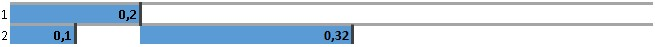
\includegraphics[scale=.8]{sections/images/second_logical_moment.jpg}
	\floatfoot{Example of the first two moments of an expansion.}%\footnotemark}
	\end{figure}
	%\footnotetext{Fonte: note}

In Figure \ref{fig:logical_units} the representation of the first and second logical moments from Figure \ref{fig:second_logical_moment} can be seen as logical units.
	\begin{figure}[H]
	\caption{Unified logical moments}
	\label{fig:logical_units}
	\centering
	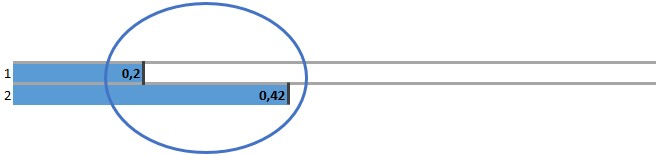
\includegraphics[scale=.8]{sections/images/logical_units.jpg}
	\floatfoot{Example of the first two unified moments of an expansion.}%\footnotemark}
	\end{figure}
	%\footnotetext{Fonte: note}

The dynamics of the theorem described above and its essential axioms of logic are cognitively observable through the mathematical construction of the natural numbers, readjusting the scale of the symbols representing each logical moment as needed by the logical expansion. Mathematics supports the addition operation, necessary in the representation of the above theorem, with Presburguer's arithmetic, which is consistent, complete, and decidable \cite{wiki_arithmetic_presburger}.

The theorem and its essential axioms of logic can also be cognitively observable by the mathematical construction of positive real numbers (represented without operations such as fractions, roots and others - the finite decimals), which is supported by the mathematical theory of the ordered field - a subset of the real numbers greater than or equal to zero and closed for the sum and product operations. The product operation and its properties are not necessary for the dynamics of the theorem and its essential axioms of logic \cite{wiki_ordered_field}. The ordered field mathematical theory is a first-order mathematical theory, with all its axioms described by first-order logic, making it complete and decidable \cite{wiki_RealClosedField}.

It is important to note that logic in its essence is not subject to mathematics, but all mathematics is restricted to logic, and therefore some of its simplest constructions may come closer to essential logic than others.

The unity present in the negation (first logical moment) and in the logical subnegations (other logical moments) is the characteristic that corresponds to the central axis of the central limit theorem. This theorem states that the sample distribution of a population approaches a normal distribution as the sample sizes increase, regardless of the shape of the population distribution. This is especially true for sample sizes greater than 30. A simple test that demonstrates this fact is the rolling of unbiased dice. The higher the dice roll number, the more likely the graph will look like the normal distribution graph \cite{statisticshowto_central_limit_theorem}. The appendix \ref{app:algorithms} explains the Distribution\_PROB algorithm in order to clarify the probabilistic essence of the central limit theorem.

It is important to note, as shown in Figure \ref{fig:trend_chart_of_normal_distribution}, that the probabilistic balance or synchronism to the right and left of the median, caused by the distribution of unified logical moments, can illustrate the doctrine of opposites of Heraclitus of Ephesus \cite{heraclitus}.
	\begin{figure}[H]
	\caption{Probabilistic synchronism of the opposite samples with respect to the median}
	\label{fig:trend_chart_of_normal_distribution}
	\centering
	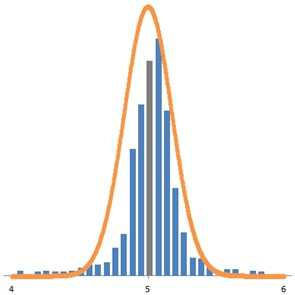
\includegraphics[scale=1]{sections/images/trend_chart_of_normal_distribution.jpg}
	\floatfoot{Example of a distribution that approximates the normal distribution.}%\footnotemark}
	\end{figure}
	%\footnotetext{Fonte: note}

In the table \ref{tab:10000_all} is the probability of the binomial distribution between 100 and 10000 samples, in line with the unified samples, Figure \ref{fig:logical_units}, or sample averages treated in the central limit theorem.

The binomial distribution behaves like the tossing of coins (heads or tails), in the case of the first row of the table, distribution of 100 samples, there are 101 possibilities, from 0 to 100, as if 100 coins were tossed adding their sides up, which can be 0 for heads and 1 for tails, for example. So if all 100 coins tossed come out heads, the sum is 0, and if they all come out tails, the sum is 100. This sum is a combination of possibilities, not a permutation, that is, in permutation [0, 1] is a possibility other than [1, 0], in combination it is 1 possibility, but with 2 probabilities of occurrence. Therefore, the sum corresponding to 100\% of the heads or 100\% of the tails corresponds to 1 possibility each, while the other sums have a higher possibility of occurrence. For this first row of the table, 100 coins, 99.994\% of all possibilities sum between 31 and 70. 

The construction of this table was performed with the general binomial probability formula (which represents a uniform distribution) using the algorithm \tiny BinomialDistribuion\_PROB \normalsize explained in Appendix \ref{app:algorithms} \cite{mathisfun_binomial_distribution}.
	\begin{align*}
	f(k;n,p) &= \binom{n}{k} p^k(1 - p)^{n-k}
	\end{align*}
The binomial distribution was used in this section of the study, but other discrete distributions could be used, such as the unbiased dice roll, and the observations in this study would remain the same because the central limit theorem is independent of the shape of the population distribution \cite{statisticsbyjim_central_limit_theorem_explainded}.
\begin{table}[H]
\caption{Probabilidade da distribuição binomial}
\floatfoot{Tabela gerada pelo algoritmo BinomialDistribuion\_PROB com a distribuição binomial de 100 a 10000. \footnotemark}
\label{tab:10000_all}
\resizebox{\textwidth}{!}{%
\begin{tabular}{cccc
>{\columncolor[HTML]{8D3CE1}}c 
>{\columncolor[HTML]{5754D6}}c 
>{\columncolor[HTML]{8FFFFB}}c c}
\hline
\cellcolor[HTML]{95ABEC} & \cellcolor[HTML]{95ABEC} & \multicolumn{2}{c}{\cellcolor[HTML]{95ABEC}} & \cellcolor[HTML]{95ABEC} & \cellcolor[HTML]{95ABEC} & \cellcolor[HTML]{95ABEC} & \cellcolor[HTML]{95ABEC} \\
\cellcolor[HTML]{95ABEC} & \cellcolor[HTML]{95ABEC} & \multicolumn{2}{c}{\cellcolor[HTML]{95ABEC}} & \cellcolor[HTML]{95ABEC} & \cellcolor[HTML]{95ABEC} & \cellcolor[HTML]{95ABEC} & \cellcolor[HTML]{95ABEC} \\
\multirow{-3}{*}{\cellcolor[HTML]{95ABEC}\textbf{Meta}} & \multirow{-3}{*}{\cellcolor[HTML]{95ABEC}\textbf{\begin{tabular}[c]{@{}c@{}}Soma do \\ Range\end{tabular}}} & \multicolumn{2}{c}{\multirow{-3}{*}{\cellcolor[HTML]{95ABEC}\textbf{Range}}} & \multirow{-3}{*}{\cellcolor[HTML]{95ABEC}\textbf{\begin{tabular}[c]{@{}c@{}}Total de \\ Amostras\end{tabular}}} & \multirow{-3}{*}{\cellcolor[HTML]{95ABEC}\textbf{\begin{tabular}[c]{@{}c@{}}Amostras \\ do Range\end{tabular}}} & \multirow{-3}{*}{\cellcolor[HTML]{95ABEC}\textbf{\begin{tabular}[c]{@{}c@{}}\% das \\ Amostras \\ do Range\end{tabular}}} & \multirow{-3}{*}{\cellcolor[HTML]{95ABEC}\textbf{\begin{tabular}[c]{@{}c@{}}Range de $\approx$ 28\% \\ das Amostras \\ do Range\end{tabular}}} \\ \hline
99,99\% & 99,994\% & 31 & 70 & \textbf{101} & \textbf{39} & \textbf{38\%} & 72,87\% \\ \hline
\cellcolor[HTML]{C0C0C0}99,99\% & \cellcolor[HTML]{C0C0C0}99,992\% & \cellcolor[HTML]{C0C0C0}73 & \cellcolor[HTML]{C0C0C0}128 & \textbf{201} & \textbf{55} & \textbf{27\%} & \cellcolor[HTML]{C0C0C0}{\color[HTML]{000000} 71,11\%} \\ \hline
99,99\% & 99,991\% & 117 & 184 & \textbf{301} & \textbf{67} & \textbf{22\%} & 72,73\% \\ \hline
\cellcolor[HTML]{C0C0C0}99,99\% & \cellcolor[HTML]{C0C0C0}99,990\% & \cellcolor[HTML]{C0C0C0}162 & \cellcolor[HTML]{C0C0C0}239 & \textbf{401} & \textbf{77} & \textbf{19\%} & \cellcolor[HTML]{C0C0C0}70,62\% \\ \hline
99,99\% & 99,991\% & 207 & 294 & \textbf{501} & \textbf{87} & \textbf{17\%} & 73,64\% \\ \hline
\cellcolor[HTML]{C0C0C0}99,99\% & \cellcolor[HTML]{C0C0C0}99,991\% & \cellcolor[HTML]{C0C0C0}253 & \cellcolor[HTML]{C0C0C0}348 & \textbf{601} & \textbf{95} & \textbf{15\%} & \cellcolor[HTML]{C0C0C0}72,96\% \\ \hline
99,99\% & 99,991\% & 299 & 402 & \textbf{701} & \textbf{103} & \textbf{14\%} & 72,69\% \\ \hline
\cellcolor[HTML]{C0C0C0}99,99\% & \cellcolor[HTML]{C0C0C0}99,990\% & \cellcolor[HTML]{C0C0C0}346 & \cellcolor[HTML]{C0C0C0}455 & \textbf{801} & \textbf{109} & \textbf{13\%} & \cellcolor[HTML]{C0C0C0}72,69\% \\ \hline
99,99\% & 99,991\% & 392 & 509 & \textbf{901} & \textbf{117} & \textbf{12\%} & 72,86\% \\ \hline
\cellcolor[HTML]{C0C0C0}99,99\% & \cellcolor[HTML]{C0C0C0}99,991\% & \cellcolor[HTML]{C0C0C0}439 & \cellcolor[HTML]{C0C0C0}562 & \textbf{1001} & \textbf{123} & \textbf{12\%} & \cellcolor[HTML]{C0C0C0}73,16\% \\ \hline
99,99\% & 99,991\% & 486 & 615 & \textbf{1101} & \textbf{129} & \textbf{11\%} & 73,54\% \\ \hline
\cellcolor[HTML]{C0C0C0}99,99\% & \cellcolor[HTML]{C0C0C0}99,991\% & \cellcolor[HTML]{C0C0C0}533 & \cellcolor[HTML]{C0C0C0}668 & \textbf{1201} & \textbf{135} & \textbf{11\%} & \cellcolor[HTML]{C0C0C0}71,45\% \\ \hline
99,99\% & 99,991\% & 580 & 721 & \textbf{1301} & \textbf{141} & \textbf{10\%} & 72,06\% \\ \hline
\cellcolor[HTML]{C0C0C0}99,99\% & \cellcolor[HTML]{C0C0C0}99,990\% & \cellcolor[HTML]{C0C0C0}628 & \cellcolor[HTML]{C0C0C0}773 & \textbf{1401} & \textbf{145} & \textbf{10\%} & \cellcolor[HTML]{C0C0C0}72,68\% \\ \hline
99,99\% & 99,991\% & 675 & 826 & \textbf{1501} & \textbf{151} & \textbf{10\%} & 73,31\% \\ \hline
\cellcolor[HTML]{C0C0C0}99,99\% & \cellcolor[HTML]{C0C0C0}99,990\% & \cellcolor[HTML]{C0C0C0}723 & \cellcolor[HTML]{C0C0C0}878 & \textbf{1601} & \textbf{155} & \textbf{9\%} & \cellcolor[HTML]{C0C0C0}71,76\% \\ \hline
99,99\% & 99,991\% & 770 & 931 & \textbf{1701} & \textbf{161} & \textbf{9\%} & 72,49\% \\ \hline
\cellcolor[HTML]{C0C0C0}99,99\% & \cellcolor[HTML]{C0C0C0}99,990\% & \cellcolor[HTML]{C0C0C0}818 & \cellcolor[HTML]{C0C0C0}983 & \textbf{1801} & \textbf{165} & \textbf{9\%} & \cellcolor[HTML]{C0C0C0}73,20\% \\ \hline
99,99\% & 99,990\% & 866 & 1035 & \textbf{1901} & \textbf{169} & \textbf{8\%} & 71,90\% \\ \hline
\cellcolor[HTML]{C0C0C0}99,99\% & \cellcolor[HTML]{C0C0C0}99,990\% & \cellcolor[HTML]{C0C0C0}914 & \cellcolor[HTML]{C0C0C0}1087 & \textbf{2001} & \textbf{173} & \textbf{8\%} & \cellcolor[HTML]{C0C0C0}72,67\% \\ \hline
99,99\% & 99,990\% & 1394 & 1607 & \textbf{3001} & \textbf{213} & \textbf{7\%} & 71,86\% \\ \hline
\cellcolor[HTML]{C0C0C0}99,99\% & \cellcolor[HTML]{C0C0C0}99,991\% & \cellcolor[HTML]{C0C0C0}1877 & \cellcolor[HTML]{C0C0C0}2124 & \textbf{4001} & \textbf{247} & \textbf{6\%} & \cellcolor[HTML]{C0C0C0}72,47\% \\ \hline
99,99\% & 99,990\% & 2363 & 2638 & \textbf{5001} & \textbf{275} & \textbf{5\%} & 72,38\% \\ \hline
\cellcolor[HTML]{C0C0C0}99,99\% & \cellcolor[HTML]{C0C0C0}99,990\% & \cellcolor[HTML]{C0C0C0}2850 & \cellcolor[HTML]{C0C0C0}3151 & \textbf{6001} & \textbf{301} & \textbf{5\%} & \cellcolor[HTML]{C0C0C0}72,75\% \\ \hline
99,99\% & 99,990\% & 3338 & 3663 & \textbf{7001} & \textbf{325} & \textbf{4\%} & 72,32\% \\ \hline
\cellcolor[HTML]{C0C0C0}99,99\% & \cellcolor[HTML]{C0C0C0}99,990\% & \cellcolor[HTML]{C0C0C0}3827 & \cellcolor[HTML]{C0C0C0}4174 & \textbf{8001} & \textbf{347} & \textbf{4\%} & \cellcolor[HTML]{C0C0C0}72,18\% \\ \hline
99,99\% & 99,990\% & 4316 & 4685 & \textbf{9001} & \textbf{369} & \textbf{4\%} & 72,23\% \\ \hline
\cellcolor[HTML]{C0C0C0}99,99\% & \cellcolor[HTML]{C0C0C0}99,990\% & \cellcolor[HTML]{C0C0C0}4806 & \cellcolor[HTML]{C0C0C0}5195 & \textbf{10001} & \textbf{389} & \textbf{3\%} & \cellcolor[HTML]{C0C0C0}72,42\% \\ \hline
\end{tabular}%
}
\end{table}
\footnotetext{O Apêndice \ref{app:algorithms} é dedicado a clarificar o algoritmo BinomialDistribuion\_PROB e validar o fórmula da probabilidade binomial geral usada por ele.}
\vspace{-8mm}
\begin{description}
   \item[Meta] Porcentagem das amostras observadas;
   \item[Soma do Range] Porcentagem que o \textbf{"Range"} atingiu a \textbf{"Meta"}, da mediana para as bordas, descentralizado;
   \item[Range] Range de amostras onde a \textbf{"Meta"} foi atingida do \textbf{"Total de Amostras"};
   \item[Total de Amostras] Exibe o range total avaliado, no caso da primeira linha da tabela o valor 101 corresponde às possibilidades de 0 a 100;
   \item[Amostras do Range] Quantidade de amostras do \textbf{"Range"};
   \item[Porcentagem das Amostras do Range] Porcentagem que o \textbf{"Range} representa do \textbf{"Total de Amostras"};
   \item[Range de $\approx$ 28\% das Amostras do Range] Esse range é  subconjunto do \textbf{"Range"}, formado a partir da mediana somando 14\% a direita e a esquerda, totalizando 28\%. Esses 28\% correspondem a aproximadamente 72\% das \textbf{"Amostras do Range"} e está por sua vez correspondem a 99,99\% da população total. O restante, que representam 72\% do tamanho do \textbf{"Range"}, correspondem a aproximadamente 28\% das amostras. Isso condiz com o Princípio de Pareto também conhecido como a regra do 80/20 e que também pode ser 70/30 ou 90/10, por exemplo \cite{wiki_pareto_principle}.
\end{description}
\bigbreak


It can be seen in Table \ref{tab:10000_all} that as the samples increase, the percentage occupied by 99.99\% of the samples \textbf{"\% of Samples in the Range"} tends to decrease more and more slowly, although the amount of samples representing this percentage tends to increase \textbf{"Samples in the Range"}.

The column of \textbf{"Range Samples"} from Table \ref{tab:10000_all}, blue arrows in the graph of Figure \ref{fig:total_comparison_chart_with_99_range}, will be getting closer and closer to the center of the graph proportionally. Although the amount of \textbf{"Range Samples"} increases, the proportion they take in \textbf{"Total Samples"} decreases. The purple arrows in the graph represent the column \textbf{"Total Samples"} of Table \ref{tab:10000_all}. 
	\begin{figure}[H]
	\caption{Comparison of total samples with a range of 99.99\% }
	\label{fig:total_comparison_chart_with_99_range}
	\centering
	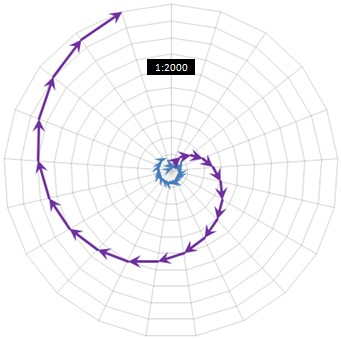
\includegraphics[scale=.9]{sections/images/total_comparison_chart_with_99_range.jpg}
	\floatfoot{The purple arrows represent the "Total Samples" column and the blue arrows the "Range Samples" column of Table \ref{tab:10000_all}. \footnotemark}
	\end{figure}
	\footnotetext{The graph in Figure \ref{fig:total_comparison_chart_with_99_range} represents the first 20 rows of Table \ref{tab:10000_all}, as they suffer equal increments of 100 samples in each row. Rows 21 onwards are incremented by 1000 samples on each row.}

At \url{https://www.mathsisfun.com/data/quincunx.html} there is a tool called Quincunx or Galton Board that dynamically exemplifies what the above pictures show. An explanation of how this tool works can be found at \url{https://www.mathsisfun.com/data/quincunx-explained.html}. 